\Problem{Vectors in a Garden}{\GardenVec}{
You visit a garden with a trail that includes the following landmarks.
\begin{itemize}
	\item Red roses at $\vec{r}_{r} = -3a\hat{x}$
	\item White roses at $\vec{r}_{w} = +4a\hat{x}$
	\item A pond at $\vec{r}_{p}=0\hat{x}$
	\item A bench at $\vec{r}_{b}=-a\hat{y}$
	\item A bridge over a creek at $\vec{r}_{c}=-a\hat{x}$
	\item A statue at $\vec{r}_{s}=+2a\hat{x}$
\end{itemize}
}
\ProblemSub{\GardenVecI}{
(1) Sketch and label the garden and its landmarks.
}
\Solution{\GardenVecISol}{

\begin{figure}[h]
	\centering
	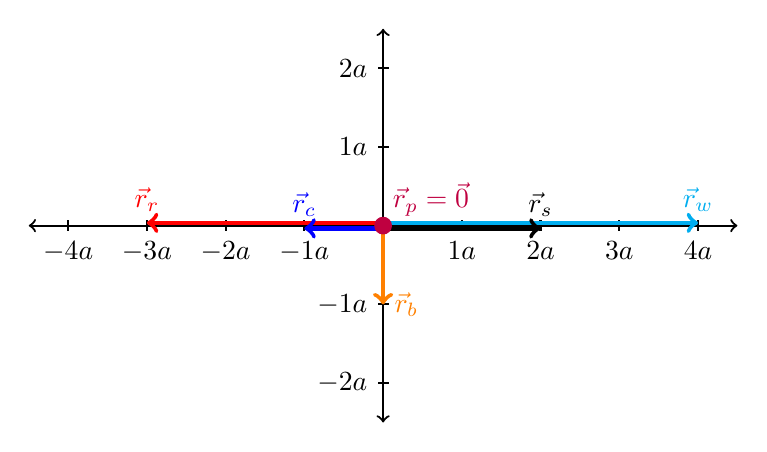
\begin{tikzpicture}
		\draw[thick,<->] (-4.5,0) -- (4.5,0);
		\foreach \x in {-4,-3,-2,-1,1,2,3,4}
			\draw[thick] (\x,2pt) -- (\x,-2pt) node[anchor=north] {$\x a$};
		\draw[thick,<->] (0,-2.5) -- (0,2.5);
		\foreach \y in {-2,-1,1,2}
			\draw[thick] (2pt,\y) -- (-2pt,\y) node[anchor=east] {$\y a$};
		\draw[ultra thick,red,->,shift={(0,1pt)}] (0,0) -- (-3,0) node[anchor=south] {$\vec{r}_{r}$};
		\draw[ultra thick,blue,->,shift={(0,-1pt)}] (0,0) -- (-1,0) node[anchor=south] {$\vec{r}_{c}$};
		\draw[ultra thick,cyan,->,shift={(0,1pt)}] (0,0) -- (4,0) node[anchor=south] {$\vec{r}_{w}$};
		\draw[ultra thick,black,->,shift={(0,-1pt)}] (0,0) -- (2,0) node[anchor=south] {$\vec{r}_{s}$};
		\draw[ultra thick,orange,->] (0,0) -- (0,-1) node[anchor=west] {$\vec{r}_{b}$};
		\filldraw[purple] (0,0) circle (3pt) node[anchor=south west] {$\vec{r}_{p}=\vec{0}$};
	\end{tikzpicture}
\end{figure}
}
\ProblemSub{\GardenVecII}{
(2) Find the following displacement vectors using both symbols and diagrams.
}
\Solution{\GardenVecIISol}{

A displacement vector, $\Delta \vec{r}$, can be thought of as the difference of the final position vector, $\vec{r}_{f}$, and the initial position vector, $\vec{r}_{i}$:
\[
\Delta\vec{r} = \vec{r}_{f}-\vec{r}_{i}.
\]
It can also be thought of as the vector that, when added to $\vec{r}_{i}$, gives you $\vec{r}_{f}$:
\[
\Delta\vec{r} = \vec{r}_{f}-\vec{r}_{i}.
\]
As such, $\Delta\vec{r}$ points from the tip of $\vec{r}_{i}$ to the tip of $\vec{r}_{f}$:
\begin{figure}[h]
	\centering
	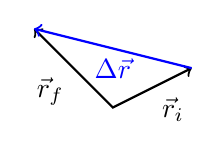
\begin{tikzpicture}
		\draw[thick,<->] (-1,1) -- (0,0) -- (1,0.5);
		\node[anchor=north east] at (-0.5,0.5) {$\vec{r}_{f}$};
		\node[anchor=north west] at (0.5,0.25) {$\vec{r}_{i}$};
		\draw[thick,blue,->] (1,0.5) -- (-1,1);
		\node[anchor=north,blue] at (0,0.75) {$\Delta\vec{r}$};
	\end{tikzpicture}
\end{figure}
}
\ProblemSub{\GardenVecIIA}{
(a) From the red roses to the white roses
}
\Solution{\GardenVecIIASol}{

\begin{figure}[h]
	\centering
	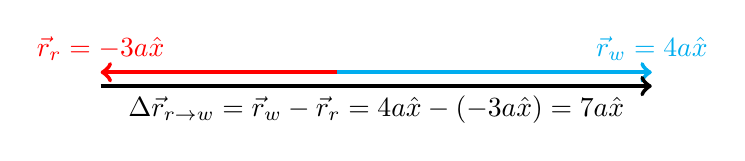
\begin{tikzpicture}
		\draw[ultra thick,red,->] (0,0) -- (-3,0) node[anchor=south] {$\vec{r}_{r}=-3a\hat{x}$};
		\draw[ultra thick,cyan,->] (0,0) -- (4,0) node[anchor=south] {$\vec{r}_{w}=4a\hat{x}$};
		\draw[ultra thick,black,->,shift={(0,-5pt)}] (-3,0) -- (4,0);
		\node[anchor=north] at (0.5,-5pt) {$\Delta\vec{r}_{r\to w} = \vec{r}_{w}-\vec{r}_{r} = 4a\hat{x} - (-3a\hat{x}) = 7a\hat{x}$};
	\end{tikzpicture}
\end{figure}
}
\ProblemSub{\GardenVecIIB}{
(b) From the pond to the red roses
}
\Solution{\GardenVecIIBSol}{

\begin{figure}[h]
	\centering
	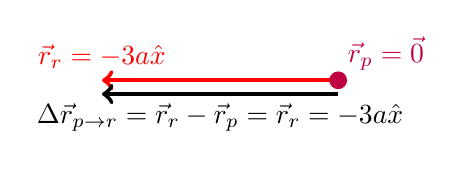
\begin{tikzpicture}
		\draw[ultra thick,red,->] (0,0) -- (-3,0) node[anchor=south] {$\vec{r}_{r}=-3a\hat{x}$};
		\filldraw[purple] (0,0) circle (3pt) node[anchor=south west] {$\vec{r}_{p}=\vec{0}$};
		\draw[ultra thick,black,->,shift={(0,-5pt)}] (0,0) -- (-3,0);
		\node[anchor=north] at (-1.5,-5pt) {$\Delta\vec{r}_{p\to r} = \vec{r}_{r}-\vec{r}_{p} = \vec{r}_{r} = -3a\hat{x}$};
	\end{tikzpicture}
\end{figure}
}
\ProblemSub{\GardenVecIIC}{
(c) From the bench to the statue
}
\Solution{\GardenVecIICSol}{

\begin{figure}[h]
	\centering
	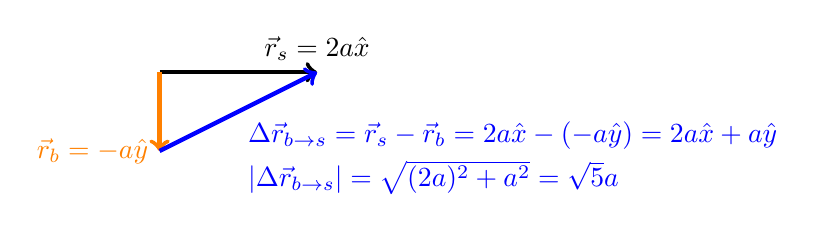
\begin{tikzpicture}
		\draw[ultra thick,black,->] (0,0) -- (2,0) node[anchor=south] {$\vec{r}_{s}=2a\hat{x}$};
		\draw[ultra thick,orange,->] (0,0) -- (0,-1) node[anchor=east] {$\vec{r}_{b}=-a\hat{y}$};
		\draw[ultra thick,blue,->] (0,-1) -- (2,0);
		\node[anchor=north west,blue] at (1,-0.5) {$\Delta\vec{r}_{b\to s} = \vec{r}_{s}-\vec{r}_{b} = 2a\hat{x} - (-a\hat{y}) = 2a\hat{x} + a\hat{y}$};
		\node[anchor=north west,blue] at (1,-1) {$\left|\Delta\vec{r}_{b\to s}\right| = \sqrt{(2a)^{2}+a^{2}} = \sqrt{5}a$};
	\end{tikzpicture}
\end{figure}
}